\documentclass[norsk,a4paper,12pt]{beamer}
\usepackage[utf8]{inputenc}
\usepackage{graphicx} %for å inkludere grafikk
\usepackage{verbatim} %for å inkludere filer med tegn LaTeX ikke liker

\title{Coupled-Cluser teori}
\author{Even Marius Nordhagen}
\institute{Universitetet i Oslo}
\date{\today}

\begin{document}
\frame{\titlepage}

  \begin{frame}
    \frametitle{Eksponensialansats}
    Den tidsuavhengige Schrödingerligningen er gitt ved
    \begin{equation}
    \hat{H}|\Psi\rangle=E|\Psi\rangle
    \end{equation}
    som kan løses eksakt med Coupled-Cluster teori. Bølgefunksjonen i Coupled-Cluster teori er som følger
    \begin{equation}
    |\Psi\rangle=e^{\hat{T}}|\Phi\rangle
    \end{equation}
    hvor $\Phi$ er referansebølgefunksjonen. 
  \end{frame}
  
  \begin{frame}
    \frametitle{Bakgrunn}
    \framesubtitle{Slaterdeterminant}
    Slaterdeterminanten for N partikler på Diracform konstruert med Hartree-Fock er gitt ved
    \begin{equation}
    |\Phi\rangle=|\phi_i(x_1)\phi_j(x_2)\cdots\phi_o(x_N)\rangle
    \end{equation}
    Orbitalfunksjoner
    \begin{equation}
    f_i(x_m)=\sum_a t_i^a\phi_a(x_m),\quad f_{ij}(x_m,x_n)=\sum_{a>b}t_{ij}^{ab}\phi_a(x_m)\phi_b(x_n)
    \end{equation}
  \end{frame}
  
  \begin{frame}
    \frametitle{Bakgrunn}
    \framesubtitle{Forbedret bølgefunksjon}
    \begin{figure}[h]
    \centering
    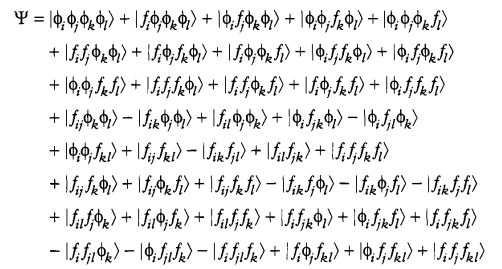
\includegraphics[width=100mm]{total_wf.png}
    \end{figure}
  \end{frame}
  
  \begin{frame}
    \frametitle{Bakgrunn}
    \framesubtitle{Orbitaloperatorer}
    \begin{equation}
    \hat{t}_i\equiv \sum_a t_i^a c_a^{\dagger}c_i,\quad \hat{t}_{ij}\equiv\sum_{a>b}t_{ij}^{ab}c_a^{\dagger}c_b^{\dagger}c_jc_i
    \end{equation}
    Som gir en total bølgefunksjon på 
    \begin{align}
    |\Psi\rangle&=\bigg(1+\sum_i\hat{t}_i+\frac{1}{2}\sum_{ij}\hat{t}_i\hat{t}_j+\frac{1}{6}\sum_{ijk}\hat{t}_i\hat{t}_j\hat{t}_k\notag\\
    &\mathrel{\phantom{=}}+\frac{1}{2}\sum_{ij}\hat{t}_{ij}
    +\frac{1}{8}\sum_{ijkl}\hat{t}_{ij}\hat{t}_{kl}+\frac{1}{24}\sum_{ijkl}\hat{t}_i\hat{t}_j\hat{t}_k\hat{t}_l\\
    &\mathrel{\phantom{=}}+\frac{1}{2}\sum_{ijk}\hat{t}_{ij}\hat{t}_k+\frac{1}{4}\sum_{ijkl}\hat{t}_{ij}\hat{t}_k\hat{t}_l\bigg)|\Phi\rangle\notag
    \end{align}
  \end{frame}
  
  \begin{frame}
    \frametitle{Bakgrunn}
    \framesubtitle{Totale clusteroperatorer}
    \begin{align}
    \hat{T}_1&=\sum_i\hat{t}_i=\sum_{ia}t_i^ac_a^{\dagger}c_i\\
    \hat{T}_2&=\frac{1}{2}\sum_{ij}\hat{t}_{ij}=\frac{1}{4}\sum_{ijab}t_{ij}^{ab}c_a^{\dagger}c_b^{\dagger}c_jc_i
    \end{align}
    som gir
    \begin{align}
    |\Psi\rangle=\bigg(&1+\hat{T}_1+\frac{1}{2!}\hat{T}_1^2+\frac{1}{3!}\hat{T}_1^3+\hat{T}_2\notag\\
    &+\frac{1}{2!}\hat{T}_2^2+\frac{1}{4!}\hat{T}_1^4+\hat{T}_2\hat{T}_1+\frac{1}{2!}\hat{T}_2\hat{T}_1^2\bigg)|\Phi\rangle
    \end{align}
  \end{frame}
  
  \begin{frame}
    \frametitle{Bakgrunn}
    \framesubtitle{Forenklet bølgerfunksjon}
    Vi definerer $\hat{T}\equiv\hat{T}_1+\hat{T}_2$:
    \begin{equation}
    |\Psi\rangle=e^{\hat{T}_1+\hat{T}_2}|\Phi\rangle\equiv e^{\hat{T}}|\Phi\rangle
    \end{equation}
    \begin{equation}
    \hat{H}e^{\hat{T}}|\Phi\rangle=Ee^{\hat{T}}|\Phi\rangle
    \end{equation}
    hvor
    \begin{equation}
    e^{\hat{T}}=1+\hat{T}+\frac{\hat{T}^2}{2!}+\frac{\hat{T}^3}{3!}+\sum_{n=4}^{\infty}\frac{\hat{T}^n}{n!}
    \end{equation}
  \end{frame}
  
  \begin{frame}
    \frametitle{Coupled Cluster ligningene}
    Ulinkede
    \begin{align}
    \langle\Phi|\hat{H}e^{\hat{T}}|\Phi\rangle&=E\\
    \langle\Phi_X|\hat{H}e^{\hat{T}}|\Phi\rangle&=0
    \end{align}
    
    Linkede
    \begin{align}
    \langle\Phi|e^{-\hat{T}}\hat{H}e^{\hat{T}}|\Phi\rangle&=E\\
    \langle\Phi_X|e^{-\hat{T}}\hat{H}e^{\hat{T}}|\Phi\rangle&=0
    \end{align}

  \end{frame}
  \begin{frame}
    \frametitle{Hausdorffs ekspansjon}
    Utvikling av $e^{-\hat{T}}\hat{H}e^{\hat{T}}$ (Hausdorffekspansjon):
    \begin{align*}
    e^{-\hat{T}}\hat{H}e^{\hat{T}}&=\hat{H}+[\hat{H},\hat{T}]+\frac{1}{2!}[[\hat{H},\hat{T}],\hat{T}]+\frac{1}{3!}[[[\hat{H},\hat{T}],\hat{T}],\hat{T}]+\cdots
    \end{align*}
	Det kan vises at dette er ekvivalent med
    \begin{align*}
    e^{-\hat{T}}\hat{H}e^{\hat{T}}&=\hat{H}+\{\hat{H}\hat{T}\}_c+\frac{1}{2}\{\{\hat{H}\hat{T}\}_c\hat{T}\}_c+\frac{1}{6}\{\{\{\hat{H}\hat{T}\}_c\hat{T}\}_c\hat{T}\}_c\\
    &\mathrel{\phantom{=}}+\hdots
    \end{align*}
  \end{frame}
  
  \begin{frame}
    \frametitle{Hamiltonianoperatoren}
    Den normalordnede elektroniske Hamiltonoperatoren er gitt ved
    \begin{equation}
    \hat{H}_N=\hat{H}-E_{ref}=\hat{F}_N+\hat{V}_N
    \end{equation}
    med
    \begin{align*}
    \hat{F}_N=\sum_{pq}f_q^p\{c_p^{\dagger}c_q\},\quad \hat{V}_N=\frac{1}{4}\sum_{pqrs}W_{rs}^{pq}\{c_p^{\dagger}c_q^{\dagger}c_sc_r\}
    \end{align*}
    For vårt tilfelle får vi
    \begin{align}
    e^{-\hat{T}}\hat{H}_Ne^{\hat{T}}&=\hat{H}_N+\{\hat{F}_N\hat{T}_1\}_c+\{\hat{V}_N\hat{T}_1\}_c+\{\hat{F}_N\hat{T}_2\}_c\notag\\
    &\mathrel{\phantom{=}}+\{\hat{V}_N\hat{T}_2\}_c+\{\hat{F}_N\hat{T}_1^2\}_c+\{\hat{V}_N\hat{T}_1^2\}_c
    \end{align}
  \end{frame}
  
  \begin{frame}
    \frametitle{Et uttrykk for energien}
    \begin{equation}
    E_{CCSD}-E_{ref}=\langle\Phi|e^{-\hat{T}}\hat{H}_Ne^{\hat{T}}|\Phi\rangle
    \end{equation}
    De leddene som bidrar er
    \begin{align*}
    \langle\Phi|\{\hat{F}_N\hat{T}_1\}_c|\Phi\rangle&=\sum_{ia}f_a^it_i^a\\
    \langle\Phi|\{\hat{V}_N\hat{T}_2\}_c|\Phi\rangle&=\frac{1}{4}\sum_{aibj}W_{ab}^{ij}t_{ij}^{ab}\\
    \frac{1}{2}\langle\Phi|\{\hat{V}_N\hat{T}_1^2\}_c|\Phi\rangle&=\frac{1}{2}\sum_{aibj}W_{ab}^{ij}t_i^at_j^b
    \end{align*}
    Energiligningen skrevet ut
    \begin{align}
    E=\sum_{ia}f_a^it_i^a+\frac{1}{4}\sum_{aibj}W_{ab}^{ij}t_{ij}^{ab}+\frac{1}{2}\sum_{aibj}W_{ab}^{ij}t_i^at_j^b
    \end{align}
  \end{frame}
  
  \begin{frame}
    \frametitle{Finne amplitudene}
    Matriseelementene for amplitudeligningene (CCSD)
    \begin{align}
    \langle\Phi_{i}^a|e^{-\hat{T}}\hat{H}e^{\hat{T}}|\Phi\rangle&=\langle\Phi|(c_i^{\dagger}c_a)e^{-\hat{T}}\hat{H}e^{\hat{T}}|\Phi\rangle=0\\
    \langle\Phi_{ij}^{ab}|e^{-\hat{T}}\hat{H}e^{\hat{T}}|\Phi\rangle&=\langle\Phi|(c_i^{\dagger}c_j^{\dagger}c_bc_a)e^{-\hat{T}}\hat{H}e^{\hat{T}}|\Phi\rangle=0
    \end{align}
    Finne amplitudene ved iterasjon
    \begin{align*}
    F_i^at_i^a+G_i^a(t)=0\quad&\Rightarrow\quad t_i^{a(k+1)}=-(F_i^a)^{-1}G_i^a(t^{(k)})\\
    F_{ij}^{ab}t_{ij}^{ab}+G_{ij}^{ab}(t)=0\quad&\Rightarrow\quad t_{ij}^{ab(k+1)}=-(F_{ij}^{ab})^{-1}G_{ij}^{ab}(t^{(k)})\\
    t_i^{a(0)}&=\cdots\\
    t_{ij}^{ab(0)}&=\cdots
    \end{align*}
  \end{frame}
% etc
\end{document}